% -----------------------------------------------
% Template for ISMIR 2014
% (based on earlier ISMIR templates)
% -----------------------------------------------

\documentclass{article}

\usepackage{ismir2014,amsmath,cite,url,graphicx}
\usepackage[utf8]{inputenc}

\title{Music Discovery in Spotify with RAMA}

\oneauthor
{José Bateira$^{1,2}$, Fabien Gouyon$^{1,2}$, Matthew Davies$^{2}$, Marcelo Caetano$^{2}$}
{$^{1}$Department of Informatics Engineering, University of Porto\\ $^{2}$Sound and Music Computing Group, INESC TEC \\ ei10133@fe.up.pt \{fgouyon,mdavies,mcaetano\}@inesctec.pt}


\begin{document}

\maketitle

\begin{abstract}
  This demo presents a Spotify App\footnote{\url{https://developer.spotify.com/technologies/apps}} of the RAMA\footnote{\url{http://rama.inescporto.pt}} system that aims to improve the way music recommendations and artist relations are shown in Spotify\footnote{\url{http://spotify.com}}.  This new version includes the majority of the existing features from RAMA\footnote{\url{http://rama.inescporto.pt/app}} including: editing the visualization parameters (to obtain more detailed graphs); adding and removing node artists (for users wishing to customize the graph); and visualization of the tags/genres that describe artists in the graph.
  The metadata used in the application is provided by the Spotify and Echonest APIs\footnote{\url{http://developer.echonest.com}}.
\end{abstract}

  \section{Music Discovery Tools in Spotify}
  \label{sec:spotify_tools}

    Spotify provides several features to allow users to discover new music such as \textit{Browse, Activity, Discovery, Radio} and \textit{Spotify Apps}.
    These features commonly present the music recommendations as a list and/or grid, however by representing the information in this way, users cannot easily understand the reasons behind the recommendations. 
    Spotify Apps offer different possibilities for users to discover new music because they rely on third-party applications. For example, Last.fm\footnote{\url{http://last.fm}} developed an application using their own recommendation system.
    However, these recommendations are displayed in a manner which is not informative for users, by again using a grid and lists. 
    The goal of creating a Spotify App for RAMA was thus to provide users with a visual representation that is more natural and intuitive than lists towards an enhanced experience of browsing music recommendations and artist relations. 

  \section{RAMA in Spotify}
  \label{sec:rama}
    \sloppy
    RAMA uses a tree graph to display a network of music artists that share similarities.
    While there are other visual-based recommendation applications (e.g., \url{http://liveplasma.com} and \url{http://musicroamer.com}).
    A downside of the applications is the use of Youtube\footnote{\url{http://youtube.com}} to stream the music tracks.
    This is not ideal given the often poor sound quality of Youttube audio. Also, Youtube is not a music oriented service thus music-related queries do not always return expected content. For example, interviews or podcasts might appear in the search results among the music videos.

    In contrast, Spotify is a music oriented service that has a large music catalogue and a high quality music content.
    It also has a very user-friendly environment that is ideal for the integration with RAMA.
    Spotify has made several tools available to develop applications\footnote{\url{http://developer.spotify.com}} integrating their services.
    Spotify Apps is the ideal choice to integrate RAMA into Spotify thus improving user experience in a more natural and intuitive way.

  \section{Main Features}
  \label{sec:features}

    \subsection{Visualization of the Artists' Map}
    \label{sub:visualization}

      RAMA's Spotify App automatically draws the map with the current playing artist as the main node, as seen in Figure~\ref{fig:spotify_app}.
      \begin{figure}[hb]
        \begin{center}
          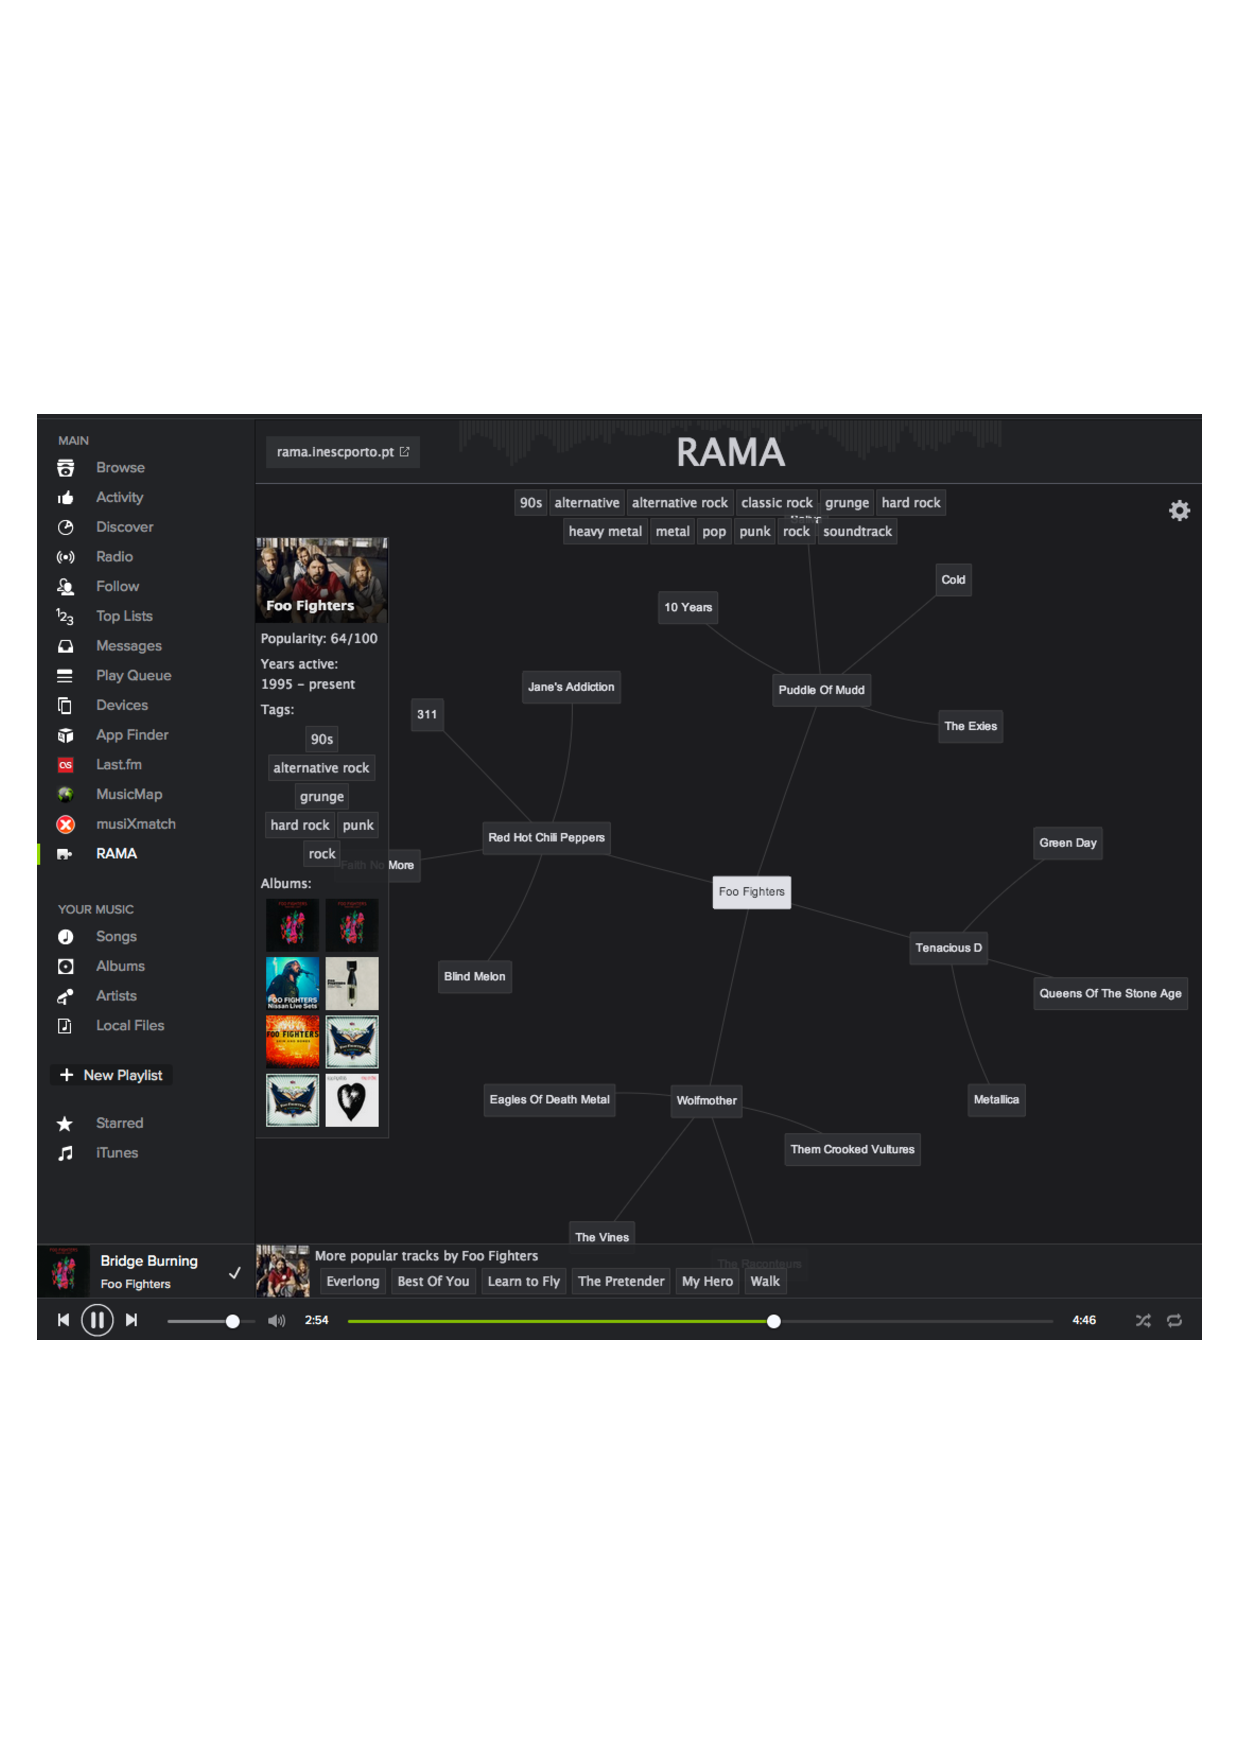
\includegraphics[width=\columnwidth]{../report/figures/graph_rootnode.pdf}
        \end{center}
        \caption{RAMA Spotify App opened inside the Spotify Desktop Client}
        \label{fig:spotify_app}
      \end{figure}
      The graph-like structure is created by recursively fetching a list of related artists from each artist using the Spotify API\footnote{\url{https://developer.spotify.com/docs/apps/api/1.0/api-models-artist.html}}.

    \subsection{Visualization Parameters}
    \label{sub:visualization_parameters}

      The visualization parameters can be personalized in the settings menu in order to create richer graphs that better match users' preferences.
      The \textit{depth} value of a graph determines how far the recursive algorithm goes when constructing the graph, such that the depth is the maximum distance between the root node and any other node in the graph.
      The \textit{branching} value of a tree graph determines the maximum number of child nodes a node can have.
      The \textit{tree mode} option indicates whether the graph to be built is a tree graph or not.
      This means that when the tree mode is on, the graph has fewer edges (which leaves the graph more clean) and so it becomes a tree graph.

    \subsection{Graph Edition}
    \label{sub:graph_edition}
      
      The available features to edit the graph are: \textit{expand node}, \textit{delete node} and \textit{create a new map}. These interactions are available in the Artist Menu (Figure~\ref{fig:artist_menu}).
      The \textit{expand node} action allows users to expand a node further (ignoring the graph's branching value).
      The \textit{delete node} action allows users to delete a node from the graph.
      These two actions are useful for when users want to construct the graph to their needs.
      The \emph{new map} action allows users create a completely new graph from a another node. This way the root node will be the selected node of the new graph.

    \subsection{Artist Menu}
    \label{sub:artist_menu}
    
      Users are able to see additional information about artists in the Artist Menu (Figure~\ref{fig:artist_menu}) such as their popularity value, albums and tags, as well as performing the expand and new map functions described in \ref{sub:graph_edition}.
      \begin{figure}[hb]
        \begin{center}
          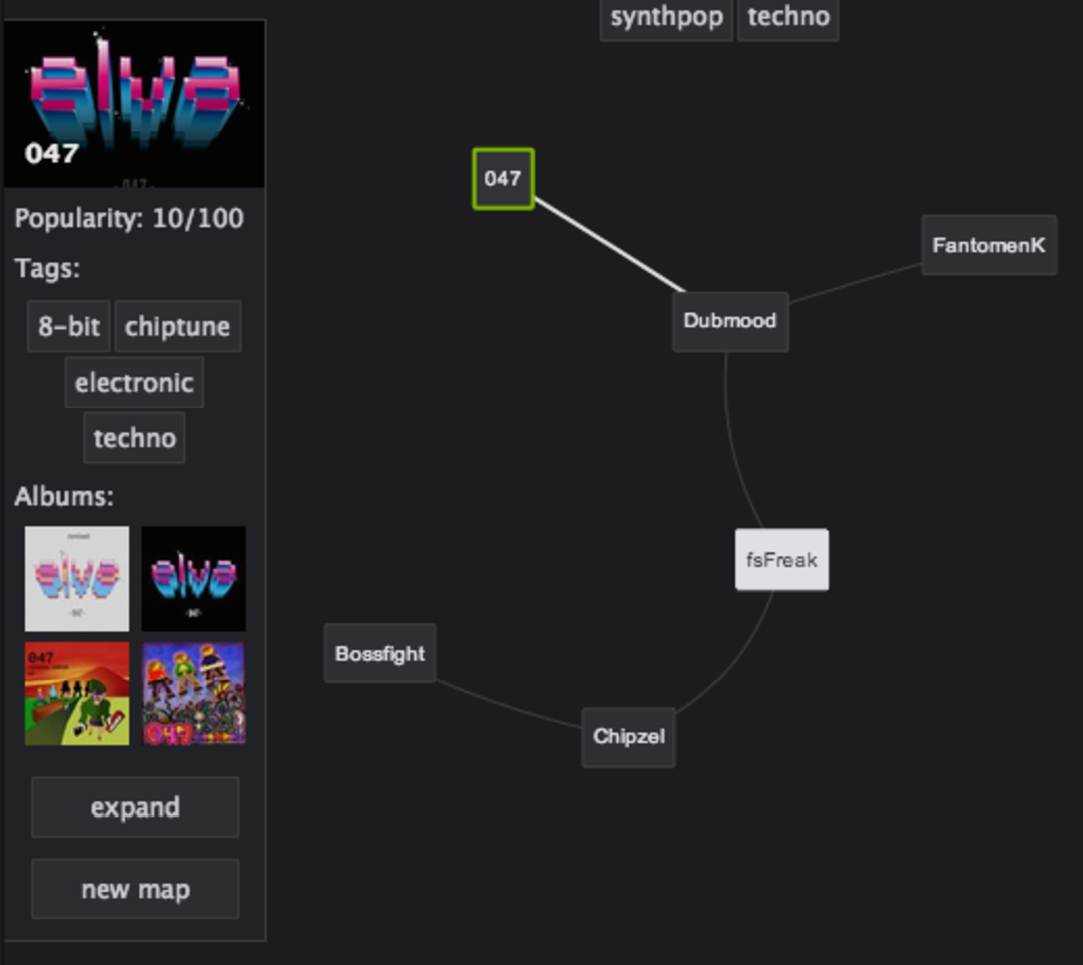
\includegraphics[width=\columnwidth]{../report/figures/artist_menu2.pdf}
        \end{center}
        \caption{Artist Menu with information about the selected node artist ``047''}
        \label{fig:artist_menu}
      \end{figure}
      When users select a node by clicking on it, the artist menu updates the displayed information.
      The popularity, the albums and the tags are metadata information retrieved from the Spotify API, although the Echonest API is also used as a fallback source for the tags  as sometimes the Spotify API only returns a small number of results.

    \subsection{Tags Overlay}
    \label{sub:tags_overlay}
    
      The tags overlay menu (Figure~\ref{fig:tags_overlay}) can enhance users' understanding of the displayed artists' nodes in terms of associated tags. These tags are the same as those used in the Artist Menu (Figure~\ref{fig:artist_menu}).
      \begin{figure}[hb]
        \begin{center}
          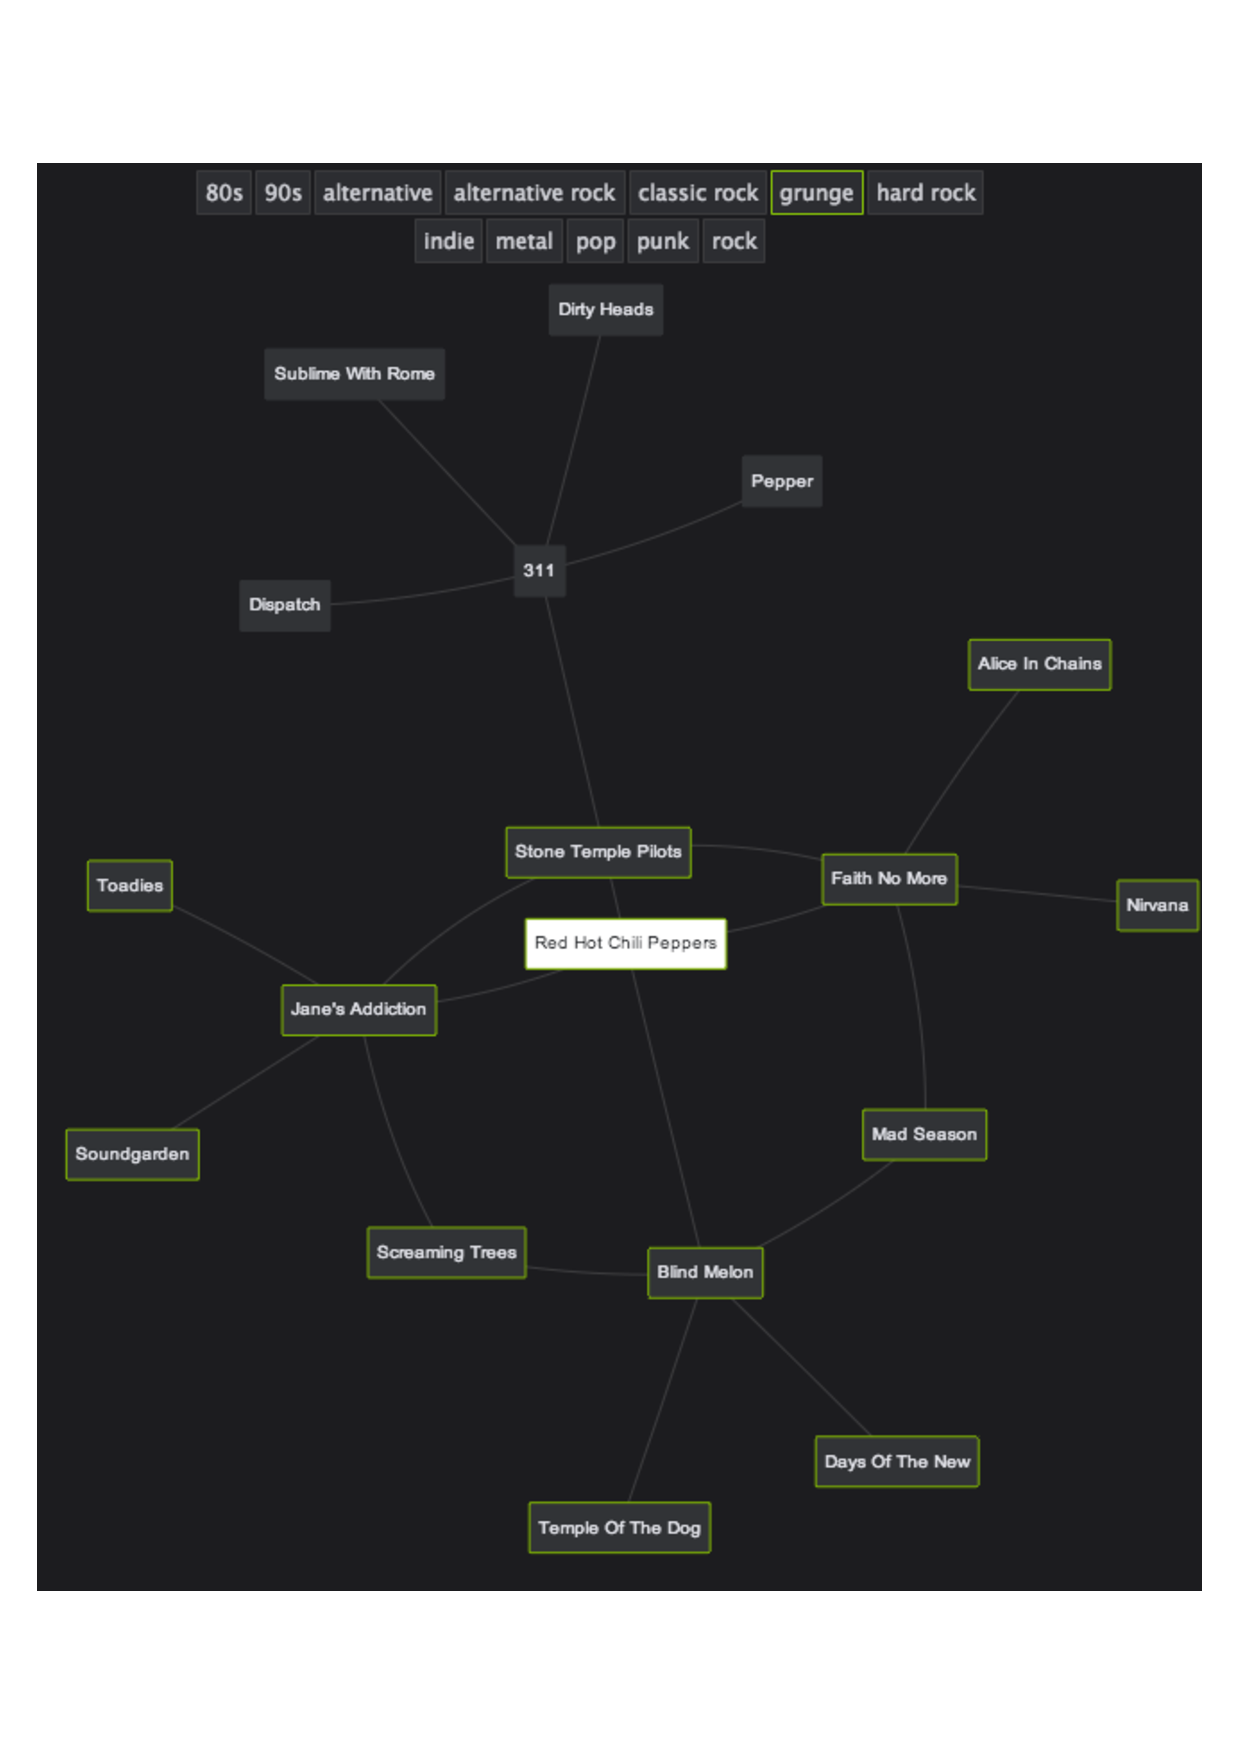
\includegraphics[width=\columnwidth]{../report/figures/tags_overlay.pdf}
        \end{center}
        \caption{Visualization of artists associated with a user-selected tag.}
        \label{fig:tags_overlay}
      \end{figure}
      They are selectable, and so, when clicked, the respective artist nodes that are described by those tags, are highlighted (as seen in Figure~\ref{fig:tags_overlay}).
      The tags shown in this menu, are just a small sample of the artists tags of the whole graph.


% \bibliography{../report/bib/myrefs}
\bibliographystyle{unstrnat}

\end{document}
